% !TeX root = ../main.tex
\documentclass[../main.tex]{subfiles}
\begin{document}
\chapter{Latex学习笔记}
\section{Latex概述}
\section{Latex安装}
\section{Latex使用}
\subsection{多文件处理}
\subsection{图片处理}
LaTeX插入图片时,常用的图片格式有:png, pdf, jpg, eps。以上四种图片格式各有优劣,其中最为显著的差异是清晰度和图片文件大小。在清晰度方面:eps是清晰度最高的,其次是pdf和png,最后是jpg。在图片的文件大小方面:与清晰度差不多一一对应,图片越清晰文件越大。
在正式开始下面的图片插入工作之前,需要注意以下几点:
\begin{enumerate}
    \item 将要使用的图片文件放在tex文件的同一个文件夹下,确保可以直接查找到文件。
    \item 图片命名中不要出现中文字符、不要空格和其他特殊符号,建议只用英文字母、下划线和简单符号。例如:本文中使用的两个图片文件名字分别为:DV\_demand.pdf, P+R\_demand.pdf。否则编译时容易出现找不到文件,或者其他奇怪的错误。
    \item 上面提到的图片格式中:编译png, pdf, jpg用 pdfLaTex,编译eps 用XeLaTex。
    \item 若图片格式不是以上四种,或者图片中空白边缘过多,可以用PS进行处理并转存为以上四种格式之一。
          插入图片需要首先在导言区引入图片宏包,
\end{enumerate}
插入图片需要首先在导言区引入图片宏包,如下:
\begin{lstlisting}[language=tex]
\usepackage{graphicx}  %插入图片的宏包
\usepackage{float}     %设置图片浮动位置的宏包
\usepackage{subfigure} %插入多图时用子图显示的宏包  
\end{lstlisting}
\subsubsection{单幅图像插入}
单幅图像插入源码如下:


\begin{lstlisting}[caption={插入单幅图像},label={插入单幅图像},language=TeX]
\begin{figure}[H] % 当前位置插入图像
    \centering
    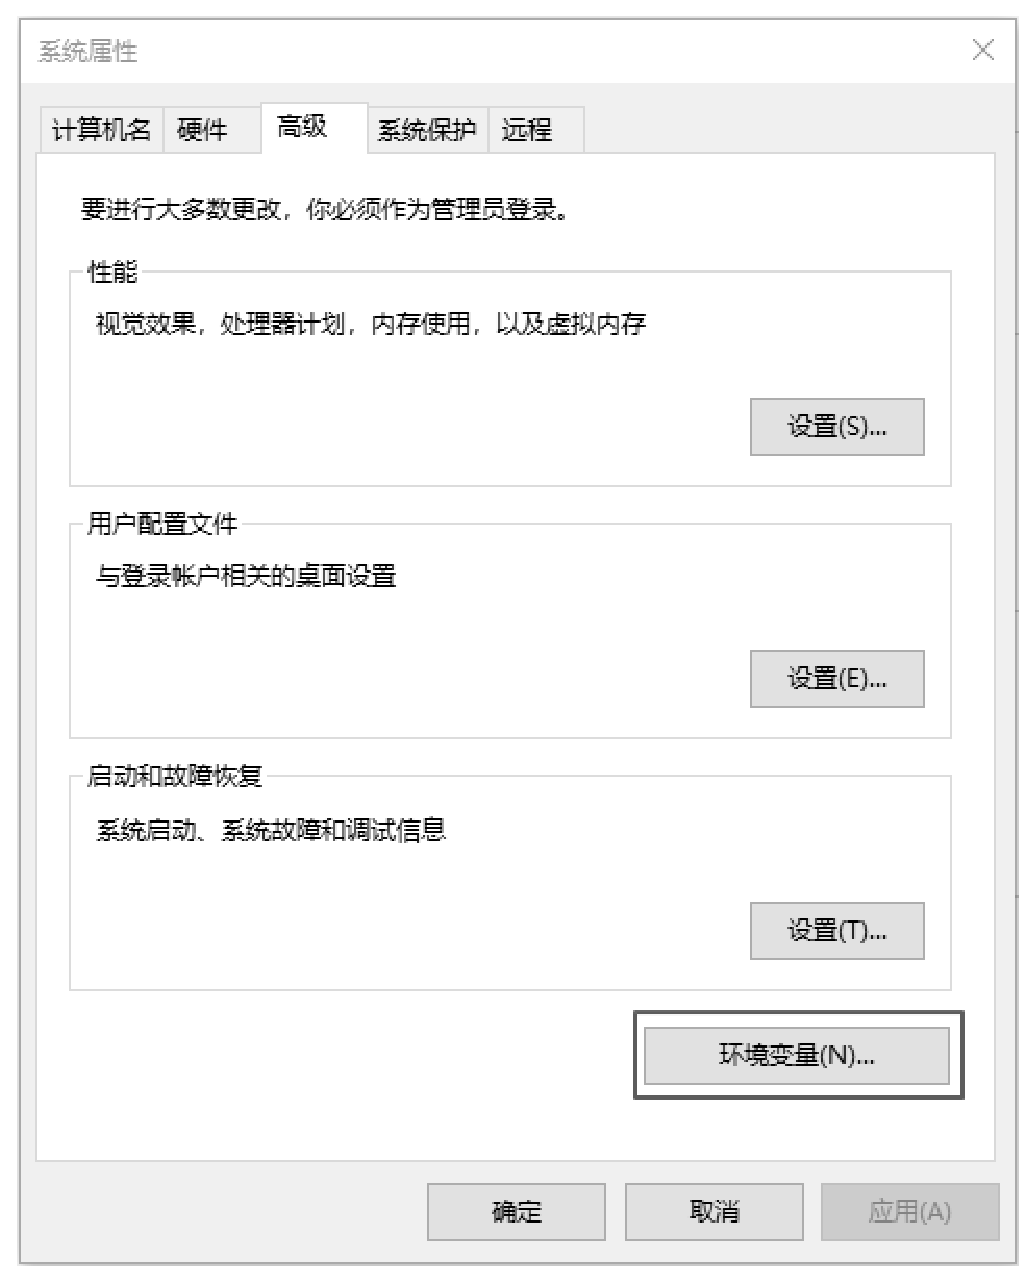
\includegraphics[width=0.5\textwidth]{set_env.eps}
    \caption{设置环境变量}
    \label{设置环境变量}
\end{figure}
\end{lstlisting}

\ref{插入单幅图像}效果如下:
\begin{figure}[H] % 当前位置插入图像
    \centering
    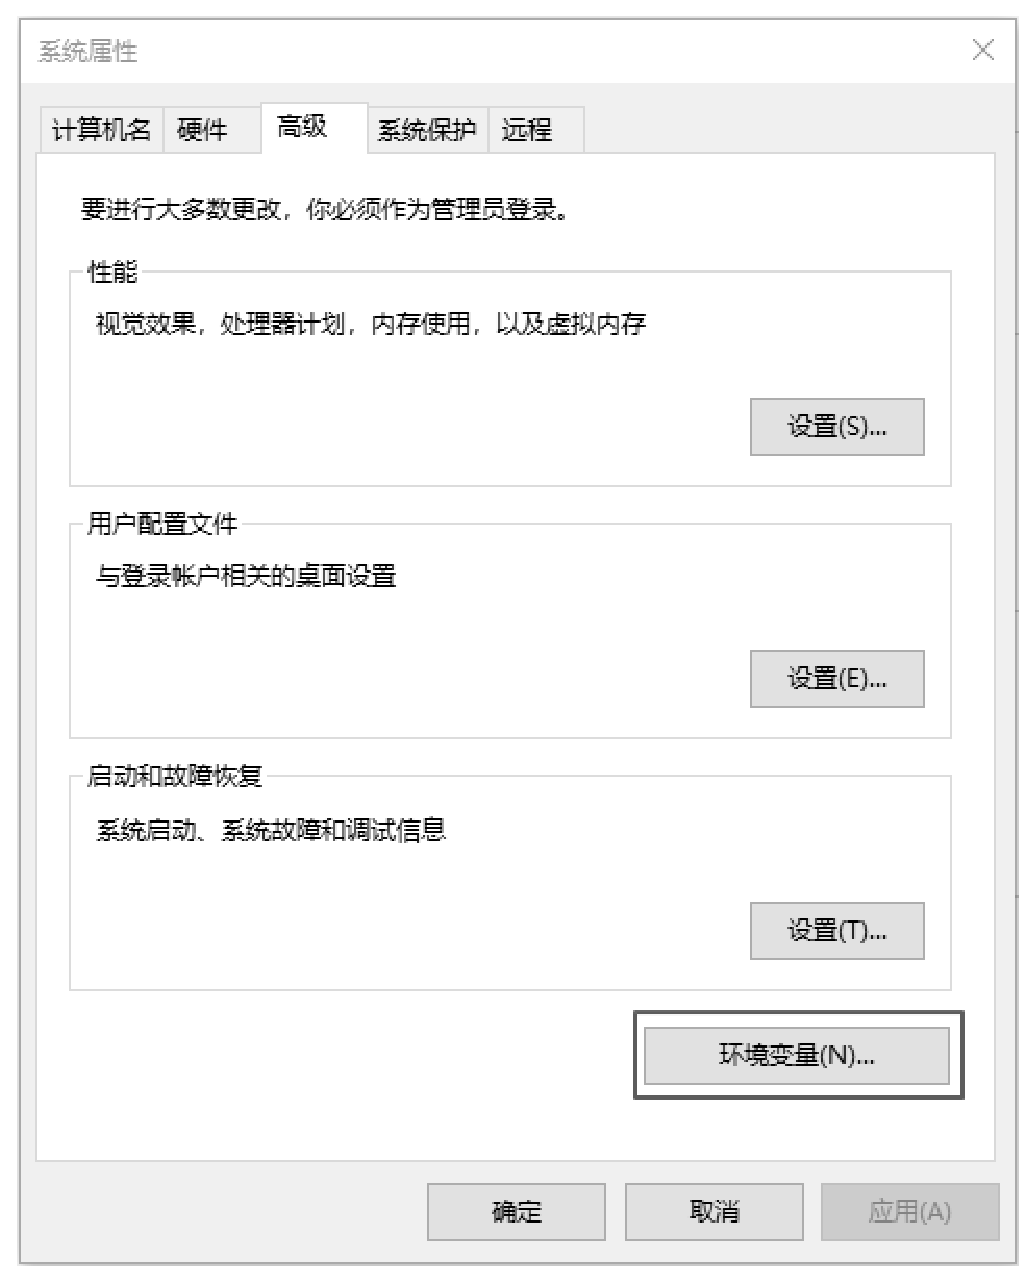
\includegraphics[width=0.5\textwidth]{set_env.eps}
    \caption{单幅图像插入}
    \label{单幅图像插入}
\end{figure}

\subsubsection{多幅图像横排插入}
多幅图像插入源码如下:
\begin{lstlisting}[caption={插入多幅图像横排},label={插入多幅图像横排},language=TeX]
%导言区插入下面三行
\usepackage{graphicx} %插入图片的宏包
\usepackage{float} %设置图片浮动位置的宏包
\usepackage{subfigure} %插入多图时用子图显示的宏包

\begin{figure}[H]
    \centering  %图片全局居中
    \subfigure[name1]{
    \label{Fig.sub.1}
    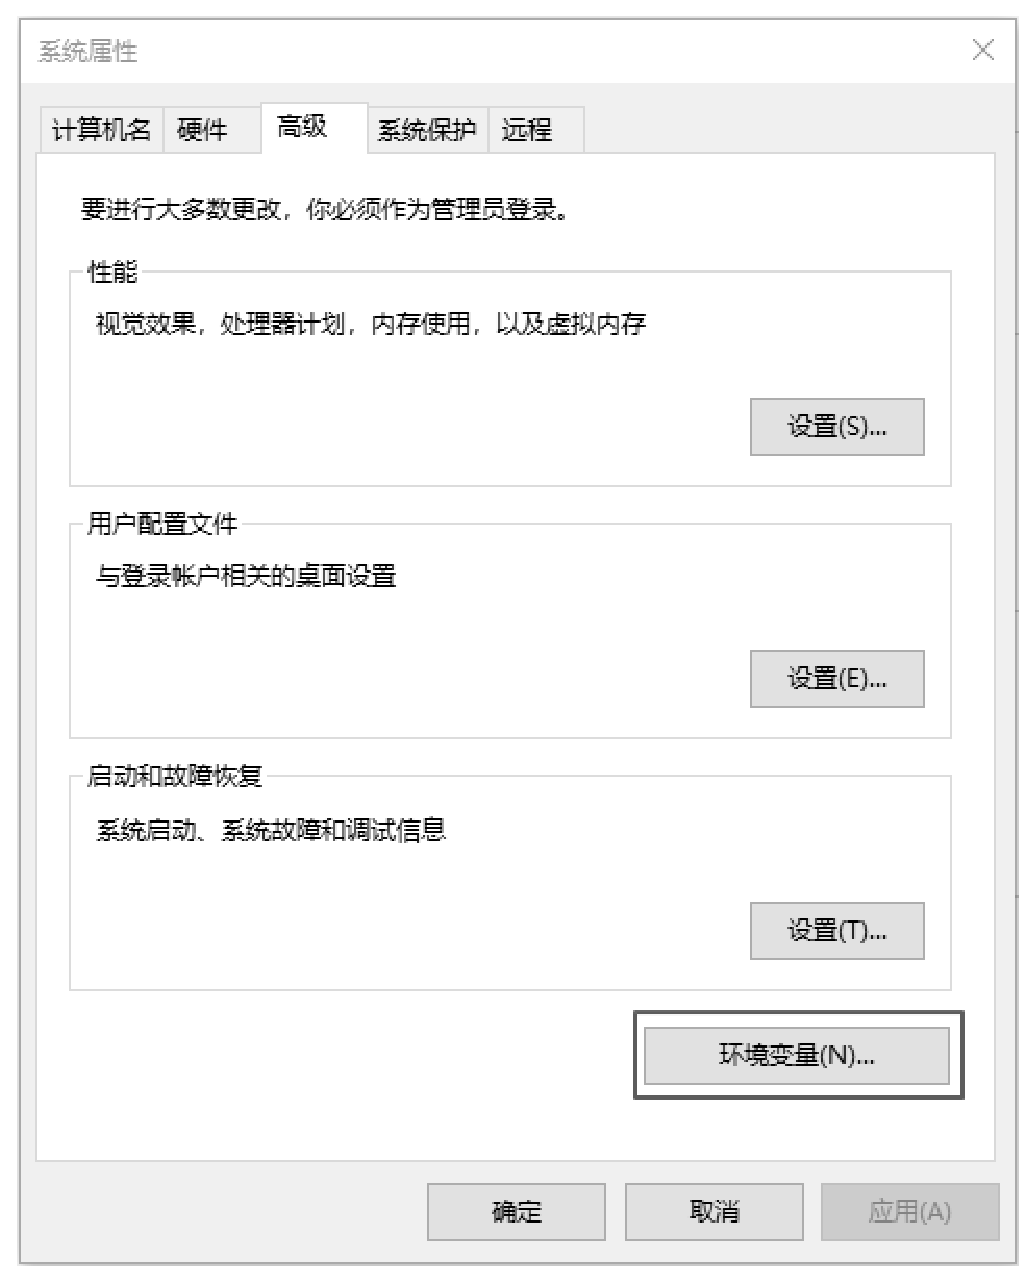
\includegraphics[width=0.45\textwidth]{set_env.eps}}
    \subfigure[name2]{
    \label{Fig.sub.2}
    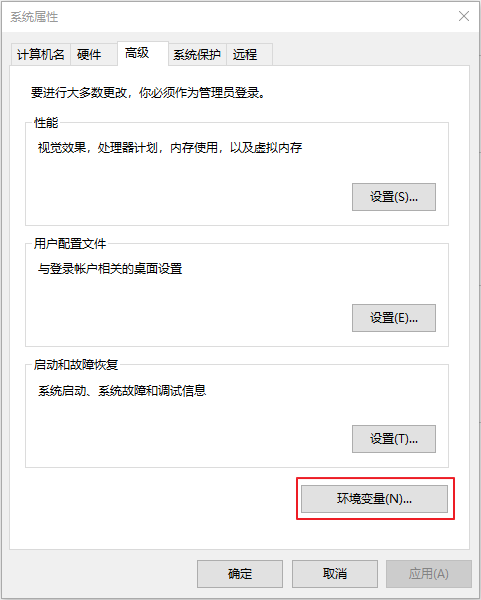
\includegraphics[width=0.45\textwidth]{set_env.png}}
    \caption{Main name}
    \label{Fig.main}
\end{figure}
\end{lstlisting}

\ref{插入多幅图像横排}效果如下:
\begin{figure}[H]
    \centering  %图片全局居中
    \subfigure[EPS图像]{
        \label{EPS图像插入}
        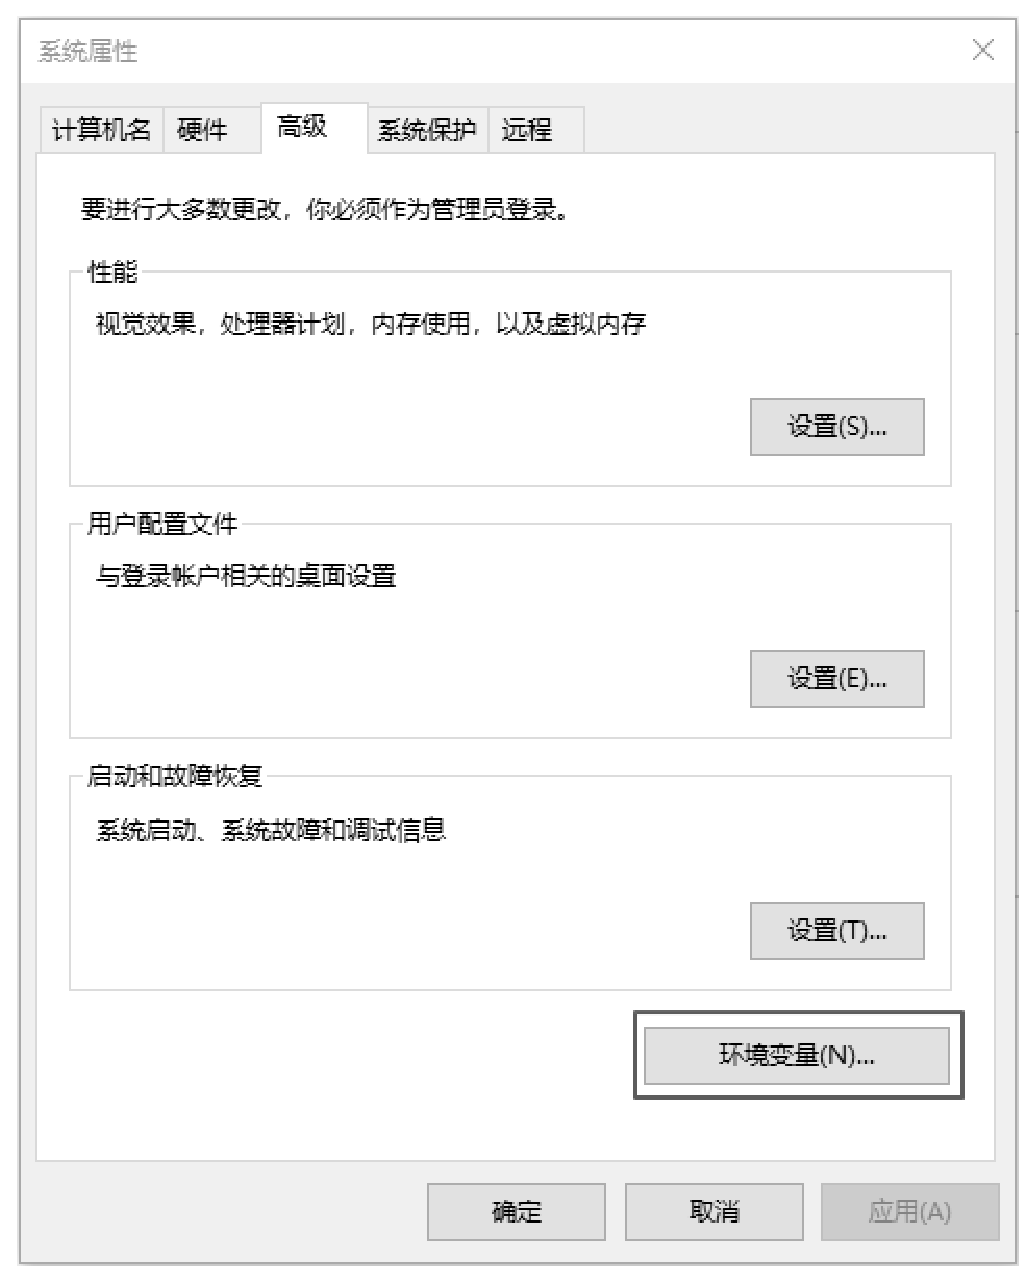
\includegraphics[width=0.45\textwidth]{set_env.eps}}
    \subfigure[PNG图像]{
        \label{PNG图像插入}
        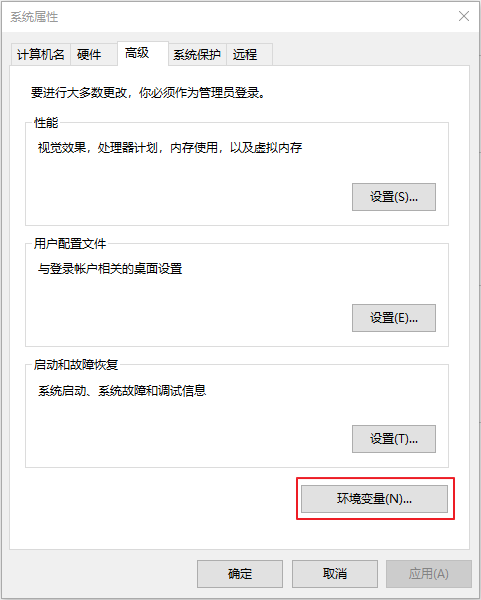
\includegraphics[width=0.45\textwidth]{set_env.png}}
    \caption{多图像插入}
    \label{多图像插入}
\end{figure}

\subsection{参考文献处理}
\subsection{插入代码}
导言区导入代码包:
\begin{lstlisting}[language=tex]
\usepackage{listings}
\usepackage{color}
\end{lstlisting}
常用的模板设置如代码\ref{Latex lstlisting}所示:
\begin{lstlisting}[caption = {Latex代码模板},language=Tex,label = {Latex lstlisting}] 
\definecolor{dkgreen}{rgb}{0,0.6,0}
\definecolor{gray}{rgb}{0.5,0.5,0.5}
\definecolor{mauve}{rgb}{0.58,0,0.82}
\lstset{ %
    language=Octave,                % the language of the code
    basicstyle=\footnotesize,       % the size of the fonts that are used for the code
    numbers=left,                   % where to put the line-numbers
    numberstyle=\tiny\color{black}, % the style that is used for the line-numbers
    stepnumber=2,                   % the step between two line-numbers. If it's 1, each line 
                                    % will be numbered
    numbersep=5pt,                  % how far the line-numbers are from the code
    backgroundcolor=\color{gray},   % choose the background color. You must add \usepackage{color}
    showspaces=false,               % show spaces adding particular underscores
    showstringspaces=false,         % underline spaces within strings
    showtabs=false,                 % show tabs within strings adding particular underscores
    frame=shadowbox,                % adds a frame around the code
    rulecolor=\color{black},        % if not set, the frame-color may be changed on line-breaks within not-black text (e.g. commens (green here))
    tabsize=2,                      % sets default tabsize to 2 spaces
    captionpos=b,                   % sets the caption-position to bottom
    breaklines=true,                % sets automatic line breaking
    breakatwhitespace=false,        % sets if automatic breaks should only happen at whitespace
    title=\lstname,                 % show the filename of files included with \lstinputlisting;
                                    % also try caption instead of title
    keywordstyle=\color{blue},      % keyword style
    commentstyle=\color{dkgreen},   % comment style
    stringstyle=\color{mauve},      % string literal style
    escapeinside={\%\*}{\*\)},      % if you want to add Latex within your code
    morekeywords={*,...}            % if you want to add more keywords to the set
    extendedchars=false             % 解决代码跨页章节标题页眉等汉字显示问题
} 
\end{lstlisting}
\end{document}